\documentclass[11pt]{article}
\usepackage{cornell-notes}
\usepackage{mathtools}
\usepackage{needspace}
\usepackage{ragged2e}
\usepackage{adjustbox}
\usepackage{tikz}
\usetikzlibrary{arrows.meta,positioning}
\tcbuselibrary{most}
\geometry{letterpaper,margin=0.72in,headheight=15pt}
\setCornellCollection{Calculus Cornell Notes}
\setCornellUnitType{Chapter}
\setCornellUnitNumber{7}
\setCornellUnitTitle{Applications of Integration}

\definecolor{Ink}{HTML}{17324D}
\definecolor{Teal}{HTML}{147D78}
\definecolor{Sky}{HTML}{DDEEF1}
\definecolor{Cue}{HTML}{EEF2F5}
\definecolor{Warm}{HTML}{FFF3D6}
\definecolor{Alert}{HTML}{9D3C32}
\definecolor{Green}{HTML}{276749}
\definecolor{Rule}{HTML}{AAB8C2}
\hypersetup{colorlinks=true,linkcolor=Ink,urlcolor=Teal,pdfborder={0 0 0}}
\setlength{\parindent}{0pt}
\setlength{\parskip}{4pt}
\setlist{nosep,leftmargin=*}
\titleformat{\section}{\Large\bfseries\color{Ink}}{}{0pt}{}[\color{Teal}\titlerule]
\titleformat{\subsection}{\large\bfseries\color{Teal}}{}{0pt}{}
\pagestyle{fancy}
\fancyhf{}
\fancyhead[L]{\small\color{Ink}\textsc{Cornell Notes}}
\fancyhead[R]{\small\color{Teal}\nouppercase{\leftmark}}
\fancyfoot[L]{\footnotesize\color{Ink}Active recall $\bullet$ Worked reasoning $\bullet$ Verification}
\fancyfoot[R]{\footnotesize\color{Ink}\thepage\ of \pageref*{LastPage}}
\renewcommand{\headrulewidth}{0.5pt}
\renewcommand{\footrulewidth}{0.4pt}
\newcolumntype{Y}{>{\RaggedRight\arraybackslash}X}
\newtcolorbox{orientationbox}{enhanced,breakable,colback=Sky,colframe=Teal,boxrule=0.7pt,arc=2mm,title=Chapter orientation,fonttitle=\bfseries}
\newtcolorbox{sectionsummarybox}{enhanced,breakable,colback=white,colframe=Teal,boxrule=0.6pt,arc=1.5mm,left=2mm,right=2mm,top=1mm,bottom=1mm,title=Section synthesis,fonttitle=\bfseries\color{Teal}}
\newtcolorbox{warningbox}{enhanced,breakable,colback=Warm,colframe=Alert,boxrule=0.7pt,arc=1.5mm,title=Common error audit,fonttitle=\bfseries}
\newtcolorbox{checkbox}{enhanced,breakable,colback=white,colframe=Green,boxrule=0.7pt,arc=1.5mm,title=Verification habit,fonttitle=\bfseries}
\newcommand{\cornellcuehead}{\rowcolor{Ink}\color{white}\bfseries Cue / recall prompt & \color{white}\bfseries Notes / reasoning \\\endhead}
\newcommand{\cornellcuerow}[2]{\rowcolor{Cue}#1 & #2 \\\addlinespace[3pt]}
\newcommand{\formula}[1]{\begin{tcolorbox}[colback=Sky,colframe=Teal,boxrule=0.5pt,arc=1mm,left=2mm,right=2mm,top=1mm,bottom=1mm]\centering\adjustbox{max width=0.97\linewidth}{$\displaystyle #1$}\end{tcolorbox}}

\title{Chapter 7: Applications of Integration\\[2mm]\large Cornell Notes}
\author{}
\date{}
\hypersetup{pdftitle={Chapter 7: Applications of Integration - Cornell Notes},pdfauthor={},pdfsubject={Calculus study notes},pdfkeywords={calculus, Cornell notes, active recall}}
\begin{document}
\maketitle
\thispagestyle{fancy}
\begin{orientationbox}
Convert geometric and physical quantities into integrals by identifying a differential element, its measure, and the accumulation interval. These notes follow the complete local section sequence (443--514) and emphasize definitions, governing results, strategy selection, and verifiable reasoning.
\end{orientationbox}

\section{Prerequisite map}
\begin{minipage}[t]{0.42\textwidth}
\textbf{Bring forward}
\begin{itemize}
\item Definite integrals
\item Substitution
\item Geometric formulas
\item Units and modeling
\end{itemize}
\end{minipage}\hfill
\begin{minipage}[t]{0.54\textwidth}
\textbf{Chapter flow}
\begin{center}
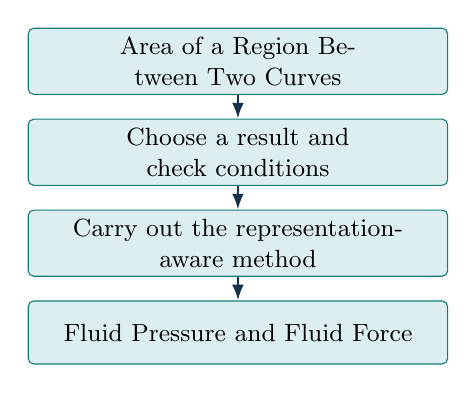
\begin{tikzpicture}[node distance=3mm, every node/.style={font=\small,align=center}, box/.style={draw=Teal,rounded corners=2pt,fill=Sky,minimum height=8mm,text width=0.42\textwidth}, arr/.style={-{Latex[length=2mm]},thick,draw=Ink}]
\node[box] (a) {Area of a Region Between Two Curves};
\node[box,below=of a] (b) {Choose a result and check conditions};
\node[box,below=of b] (c) {Carry out the representation-aware method};
\node[box,below=of c] (d) {Fluid Pressure and Fluid Force};
\draw[arr] (a)--(b); \draw[arr] (b)--(c); \draw[arr] (c)--(d);
\end{tikzpicture}
\end{center}
\end{minipage}

\section{Learning objectives}
\begin{enumerate}
\item Explain the central objects and hypotheses in 7.1 and 7.7.
\item Translate among algebraic, graphical, numerical, and verbal representations.
\item Select an appropriate formula or theorem before beginning symbolic work.
\item Carry out multi-step calculations while preserving domain, sign, orientation, and units.
\item Diagnose common errors by testing assumptions and checking the result independently.
\item Synthesize the chapter's methods into a reusable problem-solving workflow.
\end{enumerate}

\section{7.1 Area of a Region Between Two Curves}
\begin{longtable}{C N}\cornellcuehead
\cornellcuerow{What is the governing idea in 7.1?}{Area between curves accumulates nonnegative differences of outer-minus-inner or top-minus-bottom boundaries.}
\cornellcuerow{Which result should be recalled?}{\formula{A=\int_a^b[\text{top}(x)-\text{bottom}(x)]\,dx}}
\cornellcuerow{How should a problem be organized?}{Sketch, find intersections, choose vertical or horizontal slices, split where boundary order changes, and check square units.}
\cornellcuerow{What should be checked before accepting an answer?}{Confirm the hypotheses and domain, preserve units and orientation when relevant, and substitute or differentiate back into the defining relation.}
\end{longtable}
\begin{warningbox}Using one boundary order across a crossing creates cancellation instead of geometric area.\end{warningbox}
\begin{sectionsummarybox}Area between curves accumulates nonnegative differences of outer-minus-inner or top-minus-bottom boundaries. The operational habit is to sketch, find intersections, choose vertical or horizontal slices, split where boundary order changes, and check square units.\end{sectionsummarybox}
\section{7.2 Volume: The Disk Method}
\begin{longtable}{C N}\cornellcuehead
\cornellcuerow{What is the governing idea in 7.2?}{Slices perpendicular to an axis of revolution form disks or washers whose areas integrate to volume.}
\cornellcuerow{Which result should be recalled?}{\formula{V=\pi\int_a^b\bigl(R^2-r^2\bigr)\,dx}}
\cornellcuerow{How should a problem be organized?}{Draw a representative perpendicular slice, express both radii as distances to the axis, square before subtracting, and integrate over the slice coordinate.}
\cornellcuerow{What should be checked before accepting an answer?}{Confirm the hypotheses and domain, preserve units and orientation when relevant, and substitute or differentiate back into the defining relation.}
\end{longtable}
\begin{warningbox}Subtracting radii before squaring or measuring from the wrong axis changes the cross-sectional area.\end{warningbox}
\begin{sectionsummarybox}Slices perpendicular to an axis of revolution form disks or washers whose areas integrate to volume. The operational habit is to draw a representative perpendicular slice, express both radii as distances to the axis, square before subtracting, and integrate over the slice coordinate.\end{sectionsummarybox}
\section{7.3 Volume: The Shell Method}
\begin{longtable}{C N}\cornellcuehead
\cornellcuerow{What is the governing idea in 7.3?}{Slices parallel to an axis of revolution form cylindrical shells with circumference, height, and thickness.}
\cornellcuerow{Which result should be recalled?}{\formula{V=2\pi\int_a^b(\text{radius})(\text{height})\,dx}}
\cornellcuerow{How should a problem be organized?}{Choose a parallel slice, measure radius from the axis, compute outer-minus-inner height, and avoid double-counting shells.}
\cornellcuerow{What should be checked before accepting an answer?}{Confirm the hypotheses and domain, preserve units and orientation when relevant, and substitute or differentiate back into the defining relation.}
\end{longtable}
\begin{warningbox}Shell radius is a distance and may require a shift such as $|x-c|$, not simply $x$.\end{warningbox}
\begin{sectionsummarybox}Slices parallel to an axis of revolution form cylindrical shells with circumference, height, and thickness. The operational habit is to choose a parallel slice, measure radius from the axis, compute outer-minus-inner height, and avoid double-counting shells.\end{sectionsummarybox}
\section{7.4 Arc Length and Surfaces of Revolution}
\begin{longtable}{C N}\cornellcuehead
\cornellcuerow{What is the governing idea in 7.4?}{Arc length integrates infinitesimal distance; revolving a curve weights that element by circumference.}
\cornellcuerow{Which result should be recalled?}{\formula{L=\int_a^b\sqrt{1+[f'(x)]^2}\,dx,\qquad S=2\pi\int_a^b r\,ds}}
\cornellcuerow{How should a problem be organized?}{Select the parameter, compute $ds$, express the radius as a nonnegative distance, and check whether an exact antiderivative exists.}
\cornellcuerow{What should be checked before accepting an answer?}{Confirm the hypotheses and domain, preserve units and orientation when relevant, and substitute or differentiate back into the defining relation.}
\end{longtable}
\begin{warningbox}Using $dx$ in place of $ds$ ignores slope, and a signed radius can produce impossible negative area.\end{warningbox}
\begin{sectionsummarybox}Arc length integrates infinitesimal distance; revolving a curve weights that element by circumference. The operational habit is to select the parameter, compute $ds$, express the radius as a nonnegative distance, and check whether an exact antiderivative exists.\end{sectionsummarybox}
\section{7.5 Work}
\begin{longtable}{C N}\cornellcuehead
\cornellcuerow{What is the governing idea in 7.5?}{Work accumulates force along displacement; variable force and distributed lifting require a position-dependent integrand.}
\cornellcuerow{Which result should be recalled?}{\formula{W=\int_a^b F(x)\,dx}}
\cornellcuerow{How should a problem be organized?}{Define a slice or displaced element, express force at its current position, multiply by distance moved, and retain force-distance units.}
\cornellcuerow{What should be checked before accepting an answer?}{Confirm the hypotheses and domain, preserve units and orientation when relevant, and substitute or differentiate back into the defining relation.}
\end{longtable}
\begin{warningbox}Using total weight times one distance fails when different pieces move different distances.\end{warningbox}
\begin{sectionsummarybox}Work accumulates force along displacement; variable force and distributed lifting require a position-dependent integrand. The operational habit is to define a slice or displaced element, express force at its current position, multiply by distance moved, and retain force-distance units.\end{sectionsummarybox}
\section{7.6 Moments, Centers of Mass, and Centroids}
\begin{longtable}{C N}\cornellcuehead
\cornellcuerow{What is the governing idea in 7.6?}{Moments weight mass by lever arm; dividing moments by total mass locates balance coordinates.}
\cornellcuerow{Which result should be recalled?}{\formula{\bar x=\frac{M_y}{m},\qquad \bar y=\frac{M_x}{m}}}
\cornellcuerow{How should a problem be organized?}{Choose density and a differential mass element, compute total mass and signed moments, then use symmetry as an independent check.}
\cornellcuerow{What should be checked before accepting an answer?}{Confirm the hypotheses and domain, preserve units and orientation when relevant, and substitute or differentiate back into the defining relation.}
\end{longtable}
\begin{warningbox}Subscripts identify the axis about which a moment is taken; swapping them swaps centroid coordinates.\end{warningbox}
\begin{sectionsummarybox}Moments weight mass by lever arm; dividing moments by total mass locates balance coordinates. The operational habit is to choose density and a differential mass element, compute total mass and signed moments, then use symmetry as an independent check.\end{sectionsummarybox}
\section{7.7 Fluid Pressure and Fluid Force}
\begin{longtable}{C N}\cornellcuehead
\cornellcuerow{What is the governing idea in 7.7?}{Hydrostatic pressure grows with depth, so force integrates pressure over horizontal area elements.}
\cornellcuerow{Which result should be recalled?}{\formula{F=\int \rho g\,h(y)\,w(y)\,dy}}
\cornellcuerow{How should a problem be organized?}{Choose a horizontal strip, express its depth below the surface and width from geometry, then integrate pressure times area.}
\cornellcuerow{What should be checked before accepting an answer?}{Confirm the hypotheses and domain, preserve units and orientation when relevant, and substitute or differentiate back into the defining relation.}
\end{longtable}
\begin{warningbox}Using vertical position directly as depth or treating pressure as constant ignores the central variation.\end{warningbox}
\begin{sectionsummarybox}Hydrostatic pressure grows with depth, so force integrates pressure over horizontal area elements. The operational habit is to choose a horizontal strip, express its depth below the surface and width from geometry, then integrate pressure times area.\end{sectionsummarybox}

\section{Definitions and theorem register}
\small
\begin{longtable}{@{}>{\RaggedRight\arraybackslash}p{0.24\textwidth}>{\RaggedRight\arraybackslash}p{0.40\textwidth}>{\RaggedRight\arraybackslash}p{0.29\textwidth}@{}}
\toprule
\textbf{Topic} & \textbf{Meaning and conditions} & \textbf{Canonical form}\\
\midrule\endhead
7.1 Area of a Region Between Two Curves & Area between curves accumulates nonnegative differences of outer-minus-inner or top-minus-bottom boundaries. & \adjustbox{max width=\linewidth}{\(\displaystyle A=\int_a^b[\text{top}(x)-\text{bottom}(x)]\,dx\)} \\\addlinespace[2pt]
7.2 Volume: The Disk Method & Slices perpendicular to an axis of revolution form disks or washers whose areas integrate to volume. & \adjustbox{max width=\linewidth}{\(\displaystyle V=\pi\int_a^b\bigl(R^2-r^2\bigr)\,dx\)} \\\addlinespace[2pt]
7.3 Volume: The Shell Method & Slices parallel to an axis of revolution form cylindrical shells with circumference, height, and thickness. & \adjustbox{max width=\linewidth}{\(\displaystyle V=2\pi\int_a^b(\text{radius})(\text{height})\,dx\)} \\\addlinespace[2pt]
7.4 Arc Length and Surfaces of Revolution & Arc length integrates infinitesimal distance; revolving a curve weights that element by circumference. & \adjustbox{max width=\linewidth}{\(\displaystyle L=\int_a^b\sqrt{1+[f'(x)]^2}\,dx,\qquad S=2\pi\int_a^b r\,ds\)} \\\addlinespace[2pt]
7.5 Work & Work accumulates force along displacement; variable force and distributed lifting require a position-dependent integrand. & \adjustbox{max width=\linewidth}{\(\displaystyle W=\int_a^b F(x)\,dx\)} \\\addlinespace[2pt]
7.6 Moments, Centers of Mass, and Centroids & Moments weight mass by lever arm; dividing moments by total mass locates balance coordinates. & \adjustbox{max width=\linewidth}{\(\displaystyle \bar x=\frac{M_y}{m},\qquad \bar y=\frac{M_x}{m}\)} \\\addlinespace[2pt]
7.7 Fluid Pressure and Fluid Force & Hydrostatic pressure grows with depth, so force integrates pressure over horizontal area elements. & \adjustbox{max width=\linewidth}{\(\displaystyle F=\int \rho g\,h(y)\,w(y)\,dy\)} \\\addlinespace[2pt]
\bottomrule
\end{longtable}
\normalsize

\section{Formula and method sheet}
\small
\begin{longtable}{@{}>{\RaggedRight\arraybackslash}p{0.08\textwidth}>{\RaggedRight\arraybackslash}p{0.48\textwidth}>{\RaggedRight\arraybackslash}p{0.37\textwidth}@{}}
\toprule
\textbf{Sec.} & \textbf{Method sequence} & \textbf{Stop-and-check trigger}\\
\midrule\endhead
7.1 & Sketch, find intersections, choose vertical or horizontal slices, split where boundary order changes, and check square units. & Using one boundary order across a crossing creates cancellation instead of geometric area. \\\addlinespace[2pt]
7.2 & Draw a representative perpendicular slice, express both radii as distances to the axis, square before subtracting, and integrate over the slice. & Subtracting radii before squaring or measuring from the wrong axis changes the cross-sectional area. \\\addlinespace[2pt]
7.3 & Choose a parallel slice, measure radius from the axis, compute outer-minus-inner height, and avoid double-counting shells. & Shell radius is a distance and may require a shift such as $|x-c|$, not simply $x$. \\\addlinespace[2pt]
7.4 & Select the parameter, compute $ds$, express the radius as a nonnegative distance, and check whether an exact antiderivative exists. & Using $dx$ in place of $ds$ ignores slope, and a signed radius can produce impossible negative area. \\\addlinespace[2pt]
7.5 & Define a slice or displaced element, express force at its current position, multiply by distance moved, and retain force-distance units. & Using total weight times one distance fails when different pieces move different distances. \\\addlinespace[2pt]
7.6 & Choose density and a differential mass element, compute total mass and signed moments, then use symmetry as an independent check. & Subscripts identify the axis about which a moment is taken; swapping them swaps centroid coordinates. \\\addlinespace[2pt]
7.7 & Choose a horizontal strip, express its depth below the surface and width from geometry, then integrate pressure times area. & Using vertical position directly as depth or treating pressure as constant ignores the central variation. \\\addlinespace[2pt]
\bottomrule
\end{longtable}
\normalsize

\section{Common errors and diagnostic checks}
\begin{warningbox}
\begin{itemize}
\item \textbf{7.1:} Using one boundary order across a crossing creates cancellation instead of geometric area.
\item \textbf{7.2:} Subtracting radii before squaring or measuring from the wrong axis changes the cross-sectional area.
\item \textbf{7.3:} Shell radius is a distance and may require a shift such as $|x-c|$, not simply $x$.
\item \textbf{7.4:} Using $dx$ in place of $ds$ ignores slope, and a signed radius can produce impossible negative area.
\item \textbf{7.5:} Using total weight times one distance fails when different pieces move different distances.
\item \textbf{7.6:} Subscripts identify the axis about which a moment is taken; swapping them swaps centroid coordinates.
\item \textbf{7.7:} Using vertical position directly as depth or treating pressure as constant ignores the central variation.
\end{itemize}
\end{warningbox}
\begin{checkbox}
Before accepting any result: state the relevant domain; check theorem hypotheses; estimate sign and scale; preserve units and orientation; and verify by substitution, differentiation, a limiting case, or a second representation.
\end{checkbox}

\section{Chapter synthesis}
Convert geometric and physical quantities into integrals by identifying a differential element, its measure, and the accumulation interval. The chapter begins with \textbf{Area of a Region Between Two Curves} and culminates in \textbf{Fluid Pressure and Fluid Force}. Across the sequence, the most reliable workflow is to identify the mathematical object, choose a representation, state the governing result with its hypotheses, compute without dropping restrictions, and audit the answer against the original definition. Every integration application begins with the right infinitesimal element; geometry, density, units, and boundary changes determine the integrand before any antiderivative does.

\section{Self-test questions}
\begin{enumerate}
\item Explain the central distinction or object in 7.1, using both words and notation.
\item State the main formula or result from 7.2 and identify every hypothesis or restriction needed for its use.
\item Describe the problem-solving procedure for 7.3. What is the strongest independent check?
\item Compare the roles of Area of a Region Between Two Curves and Fluid Pressure and Fluid Force within this chapter.
\item Reconstruct the governing formula for 7.4 from its geometric or analytic meaning.
\item Choose one method in the chapter and explain how its output should be interpreted, including units or orientation when applicable.
\item Scenario: A student working on 7.1 produces a polished calculation but makes this error: Using one boundary order across a crossing creates cancellation instead of geometric area. Diagnose the earliest invalid step and repair the workflow.
\item Scenario: A solution in 7.2 quotes the displayed formula without checking conditions. Which conditions must be checked, and what could fail if they are absent?
\item Construct a concept map linking a representation, a governing result, a computation, and a verification check from this chapter.
\item Design a two-part test for mastery: one conceptual prompt and one calculation. State what evidence would count as a complete answer.
\end{enumerate}

\Needspace{8\baselineskip}
\section{Answer key}
\small
\begin{enumerate}
\item A complete response identifies Area between curves accumulates nonnegative differences of outer-minus-inner or top-minus-bottom boundaries. It should connect that meaning to \(A=\int_a^b[\text{top}(x)-\text{bottom}(x)]\,dx\) and state the relevant domain.
\item The organizing result is \(V=\pi\int_a^b\bigl(R^2-r^2\bigr)\,dx\). The solver must check that the quantities are defined and that the assumptions named in 7.2 hold before applying it.
\item Use this sequence: Choose a parallel slice, measure radius from the axis, compute outer-minus-inner height, and avoid double-counting shells. The strongest check is to return to the defining relation or differentiate/substitute the result, as appropriate.
\item Area of a Region Between Two Curves establishes area between curves accumulates nonnegative differences of outer-minus-inner or top-minus-bottom boundaries. Fluid Pressure and Fluid Force extends the chapter to hydrostatic pressure grows with depth, so force integrates pressure over horizontal area elements. The connection is the reuse of the same representations under a broader method.
\item The formula \(L=\int_a^b\sqrt{1+[f'(x)]^2}\,dx,\qquad S=2\pi\int_a^b r\,ds\) follows by translating the defining geometric or rate relationship into symbols; each factor records a distinct change or scale.
\item Interpretation must name what varies, with respect to what, and on which domain. A numerical value without units, sign, direction, or interval information is incomplete whenever those features are part of the modeled quantity.
\item The earliest fault is the unverified assumption described by this warning: Using one boundary order across a crossing creates cancellation instead of geometric area. Restart by following this procedure: Sketch, find intersections, choose vertical or horizontal slices, split where boundary order changes, and check square units.
\item The formula \(V=\pi\int_a^b\bigl(R^2-r^2\bigr)\,dx\) is conditional, not decorative. Check domain, differentiability or integrability as relevant, boundary or orientation requirements, and nonzero denominators before drawing a conclusion.
\item One valid map is: the representation in 7.1 identifies the object; the result in 7.2 supplies a rule; the method in 7.3 carries out the computation; the check in 7.7 tests the conclusion against its definition.
\item The conceptual prompt should require explanation of a definition and its hypotheses. The calculation should require method selection rather than direct substitution. Full evidence includes setup, justified transformations, a result, and an independent check.
\end{enumerate}
\normalsize

\section{Key-term recap}
\small
\begin{longtable}{@{}>{\RaggedRight\arraybackslash}p{0.29\textwidth}>{\RaggedRight\arraybackslash}p{0.64\textwidth}@{}}
\toprule
\textbf{Term} & \textbf{Working meaning}\\
\midrule\endhead
Area of a Region Between Two Curves & Area between curves accumulates nonnegative differences of outer-minus-inner or top-minus-bottom boundaries. \\\addlinespace[2pt]
Volume: The Disk Method & Slices perpendicular to an axis of revolution form disks or washers whose areas integrate to volume. \\\addlinespace[2pt]
Volume: The Shell Method & Slices parallel to an axis of revolution form cylindrical shells with circumference, height, and thickness. \\\addlinespace[2pt]
Arc Length and Surfaces of Revolution & Arc length integrates infinitesimal distance; revolving a curve weights that element by circumference. \\\addlinespace[2pt]
Work & Work accumulates force along displacement; variable force and distributed lifting require a position-dependent integrand. \\\addlinespace[2pt]
Moments, Centers of Mass, and Centroids & Moments weight mass by lever arm; dividing moments by total mass locates balance coordinates. \\\addlinespace[2pt]
Fluid Pressure and Fluid Force & Hydrostatic pressure grows with depth, so force integrates pressure over horizontal area elements. \\\addlinespace[2pt]
\bottomrule
\end{longtable}
\normalsize

\enlargethispage{4\baselineskip}
\begin{tcolorbox}[title=One-sentence takeaway,fonttitle=\bfseries,colback=Ink,colframe=Ink,coltext=white,coltitle=white,arc=2mm,boxrule=0pt]
\centering\bfseries Every integration application begins with the right infinitesimal element; geometry, density, units, and boundary changes determine the integrand before any antiderivative does.
\end{tcolorbox}
\end{document}
